\Variant{28.12.2025}
\QQ{1}{$\underbrace{222222\ldots222}_{50\text{ ta }2}:22$ ni hisoblang.
\Opts{$\underbrace{101010\ldots10}_{25\text{ ta }10}1$}{$\underbrace{101010\ldots10}_{24\text{ ta }10}$}{$\underbrace{101010\ldots10}_{25\text{ ta }10}$}{$\underbrace{101010\ldots10}_{24\text{ ta }10}1$}}
\QQ{2}{Kasrlarni kamayiş tartibida joylaştiring: $a=2{,}(14)$, $b=2{,}1(4)$, $c=2{,}11(4)$.
\Opts{$a>b>c$}{$b>a>c$}{$c>a>b$}{$b>c>a$}}
\QQ{3}{Fermer bozorga qovun va tarvuzni $5$ ta maşina bilan olib borayotgan bölsa va bitta maşinada faqat tarvuz yoki qovun bölsa, birinçi maşinada $300$, ikkinçi maşinada $315$, uçinçisida $330$, törtinçi maşinada $345$, beşinçisida $390$ ta mahsulot bor. Bozorkom bitta maşinani sotib bölmagunça qolganlarini sotişga ruxsat bermasdi. Bitta maşina sotib bölinganidan söng qovunlar soni tarvuzlar sonidan $3$ marta köpligi aniqlandi. Qovunlarning soni neçta?
\Opts{$945$}{$1170$}{$1035$}{$990$}}
\QQ{4}{$15$ ta köylak va $20$ ta şimning birgalikdagi narxi $950\,000$ söm. $15$ ta köylakni $28\%$ çegirma va $20$ ta şimni $20\%$ çegirma bilan birgalikda sotgan narxi $724\,000$ söm böldi. Bitta köylakning çegirmasiz narxini toping.
\Opts{$27\,000$}{$25\,000$}{$36\,000$}{$30\,000$}}
\QQ{5}{Hisoblang:
\[\frac{100^3-14^3}{\sqrt{\dfrac{100^4+14^4+114^4}2}}\]
\Opts{$86$}{$114$}{$84$}{$112$}}
\QQ{6}{Hisoblang:
\[\frac{10^2+11^2+12^2+13^2+14^2}{146}\]
\Opts{$3$}{$4$}{$5$}{$6$}}
\QQ{7}{Ifodani soddalaştiring:
\[\frac{(x-2)^4+(x-1)^2-1}{(x-2)(x-3)+2}\]
\Opts{$x^2-3x+2$}{$x^2+2x+2$}{$x^2-2x+2$}{$x^2-5x+8$}}
\QQ{8}{Arifmetik progressiyada $a_3=a_1+a_2$ va $a_1\cdot a_2\cdot a_3=384$ tengliklar örinli bölsa, $S_{10}$ ni toping.
\Opts{$220$}{$240$}{$230$}{$200$}}
\QQ{9}{Ösuvçi geometrik progressiyada $b_{10}=5$ bölsa, geometrik progressiyaning dastlabki $19$ ta hadi köpaytmasini toping.
\Opts{$5^{18}$}{$5^{19}$}{$5^{20}$}{$5^{21}$}}
\QQ{10}{Hisoblang:
\[\sqrt{\frac{666666^2}{12345654321}}\]
\Opts{$6$}{$36$}{$12$}{$4$}}
\QQ{11}{Tenglama neçta haqiqiy ildizga ega?
\[\frac{x^3}{|x|}+10x-\frac{11|x|}{|x|}=0\]
\Opts{$1$ ta}{$2$ ta}{çeksiz köp}{$3$ ta}}
\QQ{12}{$14^{\sin x}=7^{\sin x}\cdot(0{,}5)^{\cos x}$ tenglamaning $x\in\left[-4\pi;\,-\dfrac{5\pi}2\right]$ oraliqdagi yeçimlari yiğindisini toping (agar u yagona bölsa, şu ildizni toping).
\Opts{$-\dfrac{13\pi}4$}{$-\dfrac{13\pi}2$}{$-\dfrac{11\pi}4$}{$-\dfrac{9\pi}4$}}
\QQ{13}{$\sin x\cos x=\dfrac12\arcsin\left(-\dfrac{\sqrt3}2\right)$ neçta ildizga ega?
\Opts{$2$}{$3$}{$1$}{Yeçimga ega emas}}
\QQ{14}{Tenglamaning haqiqiy ildizlari köpaytmasini toping:
\[\frac23-\log_x3=\log_32\cdot\log_{32}x-\frac25\log_{\sqrt x}3\]
\Opts{$\sqrt[3]3$}{$27\sqrt[3]3$}{$27$}{$9\sqrt[3]3$}}
\QQ{15}{Agar $3(3x+4)^{20}=C_0x^{20}+C_1x^{19}+C_2x^{18}+\dots+C_{19}x+C_{20}$ tenglik örinli bölsa, $20\cdot19\cdot C_0-19\cdot18\cdot C_1+18\cdot17\cdot C_2-\ldots-3\cdot2\cdot C_{17}+C_{18}\cdot2\cdot1$ ni hisoblang.
\Opts{$11260$}{$10260$}{$11620$}{$9360$}}
\QQ{16}{Hisoblang:
\[(1+\tg7^\circ)(1+\tg8^\circ)(1+\tg37^\circ)(1+\tg38^\circ)\]
\Opts{$4$}{$2$}{$8$}{$16$}}
\QQ{17}{Tengsizlikni neçta butun son qanoatlantiradi?
\[\frac{x^2-7|x|+10}{x^2-6x+9}<0\]
\Opts{$1$ ta}{$2$ ta}{$3$ ta}{$4$ ta}}
\QQ{18}{$y=x^2-6ax+10a^2-a-6$ parabola uçining absissasi musbat, ordinatasi manfiy böladigan barça butun $a$ larning yiğindisini toping.
\Opts{$6$}{$1$}{$3$}{$4$}}
\QQ{19}{$(x,\,y)$ natural juftliklar $xy-x+2y=5$ tenglamaning yeçimi bölsa, $x+y$ ning qiymatini toping.
\Opts{$2$}{$3$}{$4$}{$5$}}
\QQ{20}{Tengsizlikni neçta butun son qanoatlantiradi?
\[\frac1{\left(\sqrt{\frac{2-x}x}-\frac{x+1}{2x}\right)^2}\ge0\]
\Opts{$0$ ta}{$1$ ta}{$2$ ta}{$3$ ta}}
\QQ{21}{$y=\dfrac{x^2-3x-4}{x^2+3x+4}$ funksiyaning qiymatlar sohasini toping.
\Opts{$y\in[-1;\,3]$}{$y\in\left[-1;\,3\dfrac47\right]$}{$y\in[1;\,3]$}{$y\in\left[1;\,3\dfrac47\right]$}}
\QQ{22}{Agar $(x^2+ax+b)(x+3)=x^3+4x^2+5x+6$ ayniyat bölsa, $a$ va $b$ ning qiymatini toping.
\Opts{$a=1;\ b=2$}{$a=2;\ b=1$}{$a=1;\ b=3$}{$a=2;\ b=3$}}
\QQ{23}{Aniq integralni hisoblang:
\[\int_0^{\frac\pi4}\frac{\sin x}{\cos^3x}\,dx\]
\Opts{$\dfrac12$}{$\dfrac14$}{$1$}{$\dfrac32$}}
\QQ{24}{$ABC$ uçburçakning tomonlari $AB=7$, $BC=13$ va $AC=15$ ga teng. Uçburçakka içki çizilgan aylanaga va uçburçakning $AB$ va $AC$ tomonlariga urinuvçi aylana çizilgan. Şu kiçik aylana radiusini toping.
\qfig{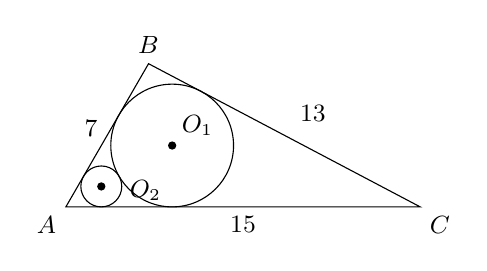
\begin{tikzpicture}[scale=0.3,font=\small]
\coordinate (A) at (0,0); \coordinate (C) at (15,0); \coordinate (B) at (3.5,6.062);
\draw (A)--(B)--(C)--cycle; \draw (4.5,2.598) circle (2.598); \draw (1.5,0.866) circle (0.866);
\fill (4.5,2.598) circle (5pt); \fill (1.5,0.866) circle (5pt);
\node[below left] at (A) {$A$}; \node[above] at (B) {$B$}; \node[below right] at (C) {$C$};
\node[above right] at (4.5,2.598) {$O_1$}; \node[right] at (2.3,0.7) {$O_2$};
\node[left] at (1.75,3.3) {$7$}; \node[above right] at (9.5,3.2) {$13$}; \node[below] at (7.5,0) {$15$};
\end{tikzpicture}}
\Opts{$\dfrac{\sqrt3}3$}{$\dfrac{3\sqrt3}2$}{$\dfrac{\sqrt3}2$}{$\dfrac{\sqrt6}2$}}
\QQ{25}{Teng yonli uçburçakning ikkita içki burçagi yiğindisi uçinçi içki burçagiga teng. Eng katta tomoniga tuşirilgan medianasi $6$ ga teng bölsa, uçburçakning yuzini toping.
\Opts{$36$}{$18$}{$48$}{$24$}}
\QQ{26}{Katta aylana radiusi $O_1A=6$ ga teng. Agar $\angle ABE=45^\circ$, $\angle CDE=60^\circ$ va $\angle O_1AC=15^\circ$ ga teng bölsa, $O_1$ va $O_2$ nuqtalar orasidagi masofani toping.
\qfig{\begin{tikzpicture}[scale=0.3,font=\small]
\coordinate (O1) at (0,0); \coordinate (O2) at (6.928,0);
\coordinate (A) at (240:6); \coordinate (E) at (330:6); \coordinate (C) at (30:6); \coordinate (B) at (115:6); \coordinate (D) at (10.392,0);
\draw (O1) circle (6); \draw (O2) circle (3.464);
\draw (B)--(A)--(C)--(D)--(E)--(B); \draw (C)--(E); \draw (O1)--(A);
\fill (O1) circle (5pt); \fill (O2) circle (5pt);
\node[above left] at (B) {$B$}; \node[below left] at (A) {$A$}; \node[above] at (C) {$C$}; \node[below] at (E) {$E$}; \node[right] at (D) {$D$};
\node[above left] at (O1) {$O_1$}; \node[below] at (O2) {$O_2$};
\node at ($(B)+(-70:1.6)$) {\scriptsize$45^\circ$}; \node at ($(A)+(70:1.7)$) {\scriptsize$15^\circ$}; \node at ($(D)+(180:1.9)$) {\scriptsize$60^\circ$};
\end{tikzpicture}}
\Opts{$6\sqrt3$}{$8$}{$4\sqrt3$}{$6\sqrt6$}}
\QQ{27}{Muntazam oltiburçakning içidagi $P$ nuqtadan tomonlarigaça bölgan masofalarning yiğindisi $18$ ga teng. Muntazam oltiburçakning yuzini toping.
\qfig{\begin{tikzpicture}[scale=1.05,font=\small]
\foreach \n/\a in {A/180,B/120,C/60,D/0,E/-60,F/-120} \coordinate (\n) at (\a:1.4);
\coordinate (P) at (-0.25,0.1);
\draw (A)--(B)--(C)--(D)--(E)--(F)--cycle;
\foreach \x/\y/\l in {A/B/A_1,B/C/B_1,C/D/C_1,D/E/D_1,E/F/E_1,F/A/F_1} {\coordinate (Q) at ($(\x)!(P)!(\y)$); \draw (P)--(Q);}
\fill (P) circle (1.2pt);
\foreach \n/\a in {A/180,B/120,C/60,D/0,E/-60,F/-120} \node at (\a:1.65) {$\n$};
\node[below right] at (P) {$P$};
\end{tikzpicture}}
\Opts{$12\sqrt3$}{$18\sqrt3$}{$24\sqrt3$}{$36$}}
\QQ{28}{$ABCD$ parallelogrammning $B$ ötmas burçagi $120^\circ$ ga teng. $BC$ tomondan $E$ nuqta olingan. $\bigl|\overrightarrow{AE}+\overrightarrow{BD}+\overrightarrow{EC}\bigr|=16$ va $\bigl|\overrightarrow{AE}-\overrightarrow{BD}+\overrightarrow{EC}\bigr|=10$ bölsa, $AED$ uçburçakning yuzini toping.
\qfig{\begin{tikzpicture}[scale=0.42,font=\small]
\coordinate (A) at (0,0); \coordinate (D) at (8,0); \coordinate (B) at (2.5,4.33); \coordinate (C) at (10.5,4.33); \coordinate (E) at (8.2,4.33);
\fill[qfill] (A)--(E)--(D)--cycle;
\draw (A)--(B)--(C)--(D)--cycle; \draw (A)--(E)--(D); \draw (B)--(D);
\node[below left] at (A) {$A$}; \node[above left] at (B) {$B$}; \node[above right] at (C) {$C$};
\node[below right] at (D) {$D$}; \node[above] at (E) {$E$};
\end{tikzpicture}}
\Opts{$15\sqrt3$}{$10\sqrt3$}{$8\sqrt3$}{$20\sqrt3$}}
\QQ{29}{$ABCD$ parallelogramm ötkir burçagi $60^\circ$ ga, diagonallari kvadratlarining nisbati $\dfrac{19}7$ ga teng. $AD>AB$ bölsa, $\dfrac{AD}{AB}$ ning qiymatini toping.
\Opts{$\dfrac32$}{$\dfrac43$}{$\dfrac53$}{$2$}}
\QQ{30}{$\alpha$ tekislikda yotmaydigan $T$ nuqtadan tekislikka $TH=4$ perpendikulyar va $\alpha$ tekislik bilan $30^\circ$ burçak taşkil qiluvçi $TA$, $TB$, $TC$ oğmalar tuşirilgan. $\angle AHB=90^\circ$, $\angle BHC=60^\circ$, $\angle AHC=150^\circ$ bölsa, $THABC$ piramida hajmini toping.
\Opts{$24+12\sqrt3$}{$32+16\sqrt3$}{$24+18\sqrt3$}{$36+12\sqrt3$}}
\QQ{31}{$A=\{x\in\mathbb N\mid x=4k+2\}$ va $B=\{x\in\mathbb N\mid x=6k+2\}$ töplamlar berilgan. $A\cap B$ töplamni toping.
\Opts{$\{x\in\mathbb N\mid x=12k+2\}$}{$\{x\in\mathbb N\mid x=24k+2\}$}{$\{x\in\mathbb N\mid x=36k+2\}$}{$\{x\in\mathbb N\mid x=48k+2\}$}}
\QQ{32}{$0$, $2$, $4$, $6$, $8$ raqamlaridan raqamlari takrorlanmaydigan uç xonali sonlar tuzildi va bir qoğozga yozildi. Ixtiyoriy bittasi tanlanganda uning $4$ ga böliniş ehtimolligini toping.
\Opts{$\dfrac56$}{$\dfrac7{10}$}{$\dfrac58$}{$\dfrac34$}}
\QQ{33}{\Moslash{Oktaedrga şar içki çizilgan. Şar hajmi $8\sqrt6\pi$ bölsa,
\par\centering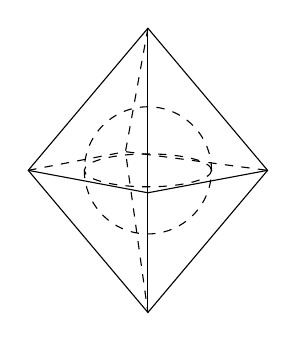
\begin{tikzpicture}[scale=0.95]
\coordinate (T) at (0,1.9); \coordinate (Bo) at (0,-1.9); \coordinate (L) at (-1.6,0); \coordinate (R) at (1.6,0); \coordinate (F) at (0,-0.3); \coordinate (K) at (-0.3,0.25);
\draw[dashed] (0,0) circle (0.85); \draw[dashed] (0,0) ellipse (0.85 and 0.22);
\draw (T)--(L)--(Bo)--(R)--cycle; \draw (T)--(F)--(Bo); \draw (L)--(F)--(R);
\draw[dashed] (L)--(K)--(R); \draw[dashed] (T)--(K)--(Bo);
\end{tikzpicture}}{A) $72$\par B) $72\sqrt2$\par C) $72\sqrt3$\par D) $36\sqrt3$\par E) $36\sqrt2$\par F) $36$}{Şar töla sirti yuzini toping ($\pi\approx3$ deb oling).}{Oktaedr töla sirti yuzini toping.}{Oktaedr hajmini toping.}}
\QQ{36}{Tenglamalar sistemasini yeçing:
\[\begin{cases}x^2+xy+y^2=133,\\ x+\sqrt{xy}+y=19\end{cases}\]
\AB{Sistemaning yeçimlari $(x_n;\,y_n)$ bölsa, $\dfrac{y_n}{x_n}$ ning eng kiçik qiymatini toping.}{$x$ va $y$ ni qanoatlantiruvçi juftliklar neçta?}}
\QQ{37}{Tenglamani yeçing:
\[\sin^3x\cdot\sin3x+\cos^3x\cdot\cos3x=\cos^36x\]
\AB{$[-\pi;\,\pi]$ oraliqda neçta yeçimga ega?}{$(0;\,2\pi)$ oraliqdagi yeçimlari yiğindisini hisoblang.}}
\QQ{38}{$g(x)=x^3+px^2+qx+d$ funksiya grafigi $OX$ öqiga $x=0$ nuqtada, $f(x)=x^3+ax^2+bx+c$ funksiya esa $x=2024$ nuqtada urinadi. $f(x)$ va $g(x)$ funksiya grafiklari $x_1=0$ va $x_2=2024$ nuqtalarda kesişadi.
\qfig{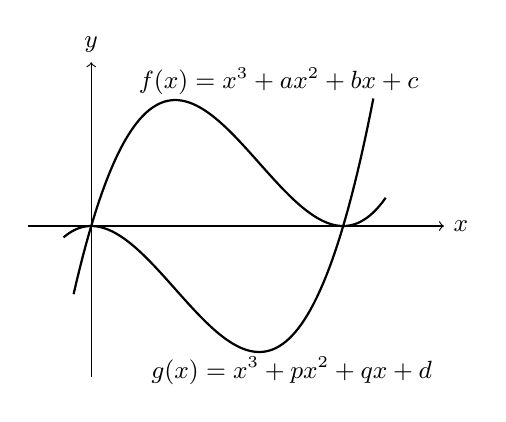
\begin{tikzpicture}[x=3.2cm,y=1.6cm,font=\small]
\draw[->] (-0.25,0)--(1.4,0) node[right] {$x$}; \draw[->] (0,-1.2)--(0,1.3) node[above] {$y$};
\draw[thick,domain=-0.07:1.17,samples=100] plot (\x,{6.75*\x*(\x-1)^2});
\draw[thick,domain=-0.11:1.12,samples=100] plot (\x,{6.75*\x*\x*(\x-1)});
\node[right] at (0.15,1.15) {$f(x)=x^3+ax^2+bx+c$}; \node[right] at (0.2,-1.15) {$g(x)=x^3+px^2+qx+d$};
\end{tikzpicture}}
\AB{$\dfrac{a\cdot p+c}{b+q+d}$ ning qiymatini toping.}{$\dfrac{g(2025)}{f(2025)}+\dfrac{g(2023)}{f(2023)}$ ning qiymatini toping.}}
\QQ{39}{$f(x)$ funksiyaning uçinçi tartibli $f'''(x)$ hosilasi mavjud. Agar
\[f(x)=\left(\frac x{1-2^x}-\frac x2\right)\cos^{2025}x\cdot\sin^{2024}x\cdot\left(\ln\sqrt{x+\sqrt{1+x^2}}\right)\]
bölsa:
\AB{$\dfrac{f'(2025)-f'(-2025)}{f'(1)+f'(-1)}$ ning qiymatini toping.}{$\dfrac{f''(2)+f''(-2)}{f'''(1)+f'''(-1)}$ ning qiymatini toping.}}
\QQ{40}{$f(x)=\sqrt{ax^2+bx+c}+d$ va $g(x)=kx^2+px+q$ funksiyalar $A(2;4)$ va $B(6;4)$ nuqtalarda kesişadi. $f(x)$ funksiya $Ox$ öqiga $C$ nuqtada urinadi va aniqlaniş sohasi $x\in[2;6]$.
\qfig{\begin{tikzpicture}[scale=0.55,font=\small]
\fill[qfill] (2,4) arc (180:0:2) -- plot[domain=6:2,samples=60] (\x,{(\x-4)^2}) -- cycle;
\draw[->] (-0.3,0)--(8,0) node[right] {$x$}; \draw[->] (0,-0.3)--(0,8) node[above] {$y$};
\draw[thick] (2,4) arc (180:0:2);
\draw[thick,domain=1.3:6.7,samples=80] plot (\x,{(\x-4)^2});
\draw[dashed] (0,6)--(4,6)--(4,0);
\node[left] at (0,6) {$6$}; \node[left] at (2,4) {$A(2;4)$}; \node[right] at (6,4) {$B(6;4)$};
\node[right] at (1.1,7.5) {$f(x)=\sqrt{ax^2+bx+c}+d$}; \node[below] at (4.2,-0.2) {$g(x)=kx^2+px+q$};
\end{tikzpicture}}
\AB{$\dfrac{k+p+q}{a+b+c+d}$ ning qiymatini toping.}{Böyalgan soha yuzini toping.}}
\QQ{41}{$ABC$ uçburçakka markazi $O$ nuqtada bölgan aylana içki çizilgan. Aylana markazidan ötuvçi asosiga parallel $EF$ kesma ötkazilgan. Agar $BEF$ uçburçak yuzi $37\frac13$ sm$^2$ ga, $AEFC$ törtburçak yuzi esa $46\frac23$ sm$^2$ ga teng va $AC=14$ sm bölsa, quyidagi topşiriqlarni bajaring.
\qfig{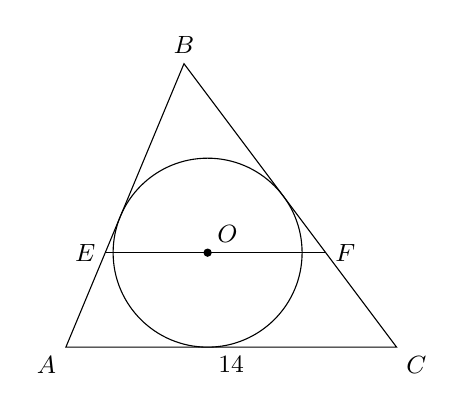
\begin{tikzpicture}[scale=0.3,font=\small]
\coordinate (A) at (0,0); \coordinate (C) at (14,0); \coordinate (B) at (5,12); \coordinate (O) at (6,4); \coordinate (E) at (1.667,4); \coordinate (F) at (11,4);
\draw (A)--(B)--(C)--cycle; \draw (O) circle (4); \draw (E)--(F); \fill (O) circle (5pt);
\node[below left] at (A) {$A$}; \node[above] at (B) {$B$}; \node[below right] at (C) {$C$}; \node[left] at (E) {$E$}; \node[right] at (F) {$F$};
\node[above right] at (O) {$O$}; \node[below] at (7,0) {$14$};
\end{tikzpicture}}
\AB{Aylana radiusini toping.}{$AEFC$ törtburçak perimetrini toping.}}
\QQ{42}{$ABCD$ trapetsiyada $A$ va $B$ burçak bissektrisalari $G$ nuqtada, $B$ va $C$ burçak bissektrisalari $E$ nuqtada, $C$ va $D$ burçak bissektrisalari $H$ nuqtada, $A$ va $D$ burçak bissektrisalari $P$ nuqtada kesişadi. $ABCD$ trapetsiyaning $AB$ va $CD$ yon tomonlari mos ravişda $5$ va $9$ ga teng va $E$ nuqta esa $AD$ tomonda yotadi. Agar $G$ va $H$ nuqtalar orqali ötkazilgan töğri çiziq $AB$ tomonni $M$ nuqtada, $CD$ tomonni esa $N$ nuqtada kesib ötsa,
\qfig{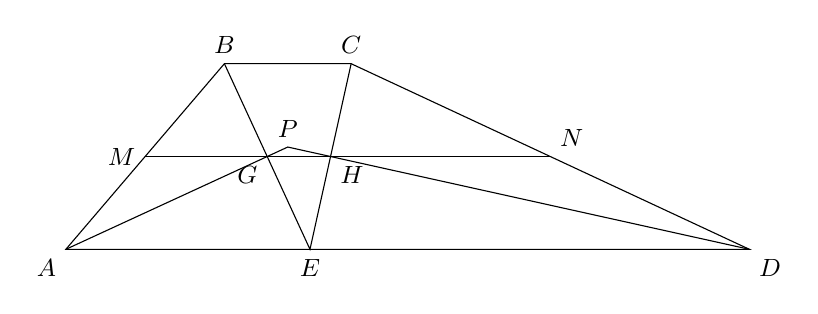
\begin{tikzpicture}[scale=0.62,font=\small]
\coordinate (A) at (0.000,0.000); \coordinate (B) at (3.247,3.802); \coordinate (C) at (5.843,3.802); \coordinate (D) at (14.000,0.000); \coordinate (E) at (5.000,0.000); \coordinate (G) at (4.124,1.901); \coordinate (H) at (5.421,1.901); \coordinate (P) at (4.545,2.095); \coordinate (M) at (1.624,1.901); \coordinate (N) at (9.921,1.901);
\draw (A)--(B)--(C)--(D)--cycle; \draw (B)--(E)--(C); \draw (A)--(P)--(D); \draw (M)--(N);
\node[below left] at (A) {$A$}; \node[above] at (B) {$B$}; \node[above] at (C) {$C$}; \node[below right] at (D) {$D$}; \node[below] at (E) {$E$};
\node[below left] at (G) {$G$}; \node[below right] at (H) {$H$}; \node[above] at (P) {$P$}; \node[left] at (M) {$M$}; \node[above right] at (N) {$N$};
\end{tikzpicture}}
\AB{$\dfrac{CN}{ND}$ ning qiymatini toping.}{$PH:GE=3:7$ bölsa, $GP:HE$ ning qiymatini toping.}}
\QQ{43}{$ABC$ uçburçakka radiusi $2\sqrt3$ ga teng bölgan aylana taşqi çizilgan. $ABC$ uçburçakning $AB$ va $BC$ tomonlari örtalaridan mos ravişda $K$ va $F$ nuqtalar olingan. Aylanaga $K$ va $F$ nuqtalardan ötuvçi $MN$ vatar ötkazilgan. Agar $ABC$ uçburçakning $AB$ tomoni $4$ ga, $BC$ tomoni esa $6$ ga teng va $\angle BAC=60^\circ$ bölsa,
\qfig{\begin{tikzpicture}[scale=0.55,font=\small]
\coordinate (O) at (0,0); \coordinate (A) at (-3.449,-0.318); \coordinate (C) at (3.449,-0.318); \coordinate (B) at (-1.449,3.146);
\coordinate (K) at ($(A)!0.5!(B)$); \coordinate (F) at ($(B)!0.5!(C)$); \coordinate (M) at (-3.162,1.414); \coordinate (N) at (3.162,1.414);
\draw (O) circle (3.464); \draw (A)--(B)--(C)--cycle; \draw (M)--(N); \draw (O)--(C); \fill (O) circle (2.5pt);
\node[left] at (A) {$A$}; \node[above] at (B) {$B$}; \node[right] at (C) {$C$}; \node[left] at (M) {$M$}; \node[right] at (N) {$N$};
\node[below right] at (K) {$K$}; \node[above right] at (F) {$F$}; \node[above] at (O) {$O$};
\node[above] at (1.7,-0.15) {$2\sqrt3$}; \node at ($(A)+(30:0.9)$) {\scriptsize$60^\circ$};
\end{tikzpicture}}
\AB{$O$ va $F$ nuqtalar orasidagi masofa neçaga teng?}{$MN$ ning uzunligini toping.}}
\QQ{44}{Balandligi $4\sqrt3$ ga teng $SABCDEF$ piramida berilgan. Piramidaning asosi $ABCDEF$ oltiburçak bölib, uning barça burçaklari teng. Agar $AB=1$, $BC=4$, $CD=2$ va $DE=4$ bölsa,
\AB{$ABCDEF$ oltiburçak perimetrini toping.}{Piramida hajmini toping.}}
\QQ{45}{Kondan yölgaça bölgan masofa ($AD$) $8$ km. Yuk maşinasi yuk bilan kondan zavodgaça boriş uçun dala böylab $8$ km/soat tezlik bilan, $DH$ yöl böylab esa $10$ km/soat tezlik bilan harakatlanadi. Yuk maşinasi yuksiz zavoddan konga borişda ($DH$) yöl böylab $20$ km/soat tezlik bilan, dala böylab esa $12$ km/soat tezlik bilan harakatlanadi.
\qfig{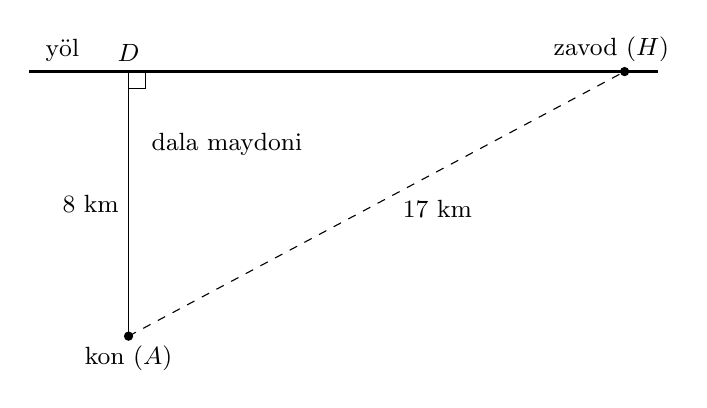
\begin{tikzpicture}[scale=0.42,font=\small]
\draw[very thick] (-3,0)--(16,0); \draw (0,0)--(0,-8); \draw[dashed] (0,-8)--(15,0);
\draw (0,0) rectangle (0.5,-0.5); \fill (0,-8) circle (4pt); \fill (15,0) circle (4pt);
\node[above] at (-2,0) {yöl}; \node[above] at (0,0) {$D$}; \node[above] at (14.6,0) {zavod ($H$)}; \node[below] at (0,-8) {kon ($A$)};
\node[left] at (0,-4) {$8$ km}; \node[below right] at (8,-3.6) {$17$ km}; \node[right] at (0.4,-2.2) {dala maydoni};
\end{tikzpicture}}
\AB{Yuk bilan kondan zavodga borişda qanday eng qisqa vaqt (daqiqa) sarflaydi?}{Yuksiz qaytişda qanday eng qisqa vaqt (daqiqa) sarflanadi?}}
\Javoblar{D B C D A C A A B A A A D B B A C C B B B A A C A C B B A B A C A C B}{%
\OK{36}{$\dfrac49$}{$2$}\OK{37}{$9$}{$7\pi$}\OK{38}{$2$}{$2$}\OK{39}{$0$}{$0$}\OK{40}{$-9$}{$2\pi+\dfrac{32}3$}%
\OK{41}{$4$}{$\dfrac{98}3$}\OK{42}{$1$}{$\dfrac5{21}$}\OK{43}{$\sqrt3$}{$2\sqrt{10}$}\OK{44}{$17$}{$43$}\OK{45}{$126$}{$77$}}
